% Options for packages loaded elsewhere
\PassOptionsToPackage{unicode}{hyperref}
\PassOptionsToPackage{hyphens}{url}
\PassOptionsToPackage{dvipsnames,svgnames,x11names}{xcolor}
%
\documentclass[
]{article}
\usepackage{amsmath,amssymb}
\usepackage{iftex}
\ifPDFTeX
  \usepackage[T1]{fontenc}
  \usepackage[utf8]{inputenc}
  \usepackage{textcomp} % provide euro and other symbols
\else % if luatex or xetex
  \usepackage{unicode-math} % this also loads fontspec
  \defaultfontfeatures{Scale=MatchLowercase}
  \defaultfontfeatures[\rmfamily]{Ligatures=TeX,Scale=1}
\fi
\usepackage{lmodern}
\ifPDFTeX\else
  % xetex/luatex font selection
\fi
% Use upquote if available, for straight quotes in verbatim environments
\IfFileExists{upquote.sty}{\usepackage{upquote}}{}
\IfFileExists{microtype.sty}{% use microtype if available
  \usepackage[]{microtype}
  \UseMicrotypeSet[protrusion]{basicmath} % disable protrusion for tt fonts
}{}
\makeatletter
\@ifundefined{KOMAClassName}{% if non-KOMA class
  \IfFileExists{parskip.sty}{%
    \usepackage{parskip}
  }{% else
    \setlength{\parindent}{0pt}
    \setlength{\parskip}{6pt plus 2pt minus 1pt}}
}{% if KOMA class
  \KOMAoptions{parskip=half}}
\makeatother
\usepackage{xcolor}
\usepackage[margin=1in]{geometry}
\usepackage{color}
\usepackage{fancyvrb}
\newcommand{\VerbBar}{|}
\newcommand{\VERB}{\Verb[commandchars=\\\{\}]}
\DefineVerbatimEnvironment{Highlighting}{Verbatim}{commandchars=\\\{\}}
% Add ',fontsize=\small' for more characters per line
\usepackage{framed}
\definecolor{shadecolor}{RGB}{248,248,248}
\newenvironment{Shaded}{\begin{snugshade}}{\end{snugshade}}
\newcommand{\AlertTok}[1]{\textcolor[rgb]{0.94,0.16,0.16}{#1}}
\newcommand{\AnnotationTok}[1]{\textcolor[rgb]{0.56,0.35,0.01}{\textbf{\textit{#1}}}}
\newcommand{\AttributeTok}[1]{\textcolor[rgb]{0.13,0.29,0.53}{#1}}
\newcommand{\BaseNTok}[1]{\textcolor[rgb]{0.00,0.00,0.81}{#1}}
\newcommand{\BuiltInTok}[1]{#1}
\newcommand{\CharTok}[1]{\textcolor[rgb]{0.31,0.60,0.02}{#1}}
\newcommand{\CommentTok}[1]{\textcolor[rgb]{0.56,0.35,0.01}{\textit{#1}}}
\newcommand{\CommentVarTok}[1]{\textcolor[rgb]{0.56,0.35,0.01}{\textbf{\textit{#1}}}}
\newcommand{\ConstantTok}[1]{\textcolor[rgb]{0.56,0.35,0.01}{#1}}
\newcommand{\ControlFlowTok}[1]{\textcolor[rgb]{0.13,0.29,0.53}{\textbf{#1}}}
\newcommand{\DataTypeTok}[1]{\textcolor[rgb]{0.13,0.29,0.53}{#1}}
\newcommand{\DecValTok}[1]{\textcolor[rgb]{0.00,0.00,0.81}{#1}}
\newcommand{\DocumentationTok}[1]{\textcolor[rgb]{0.56,0.35,0.01}{\textbf{\textit{#1}}}}
\newcommand{\ErrorTok}[1]{\textcolor[rgb]{0.64,0.00,0.00}{\textbf{#1}}}
\newcommand{\ExtensionTok}[1]{#1}
\newcommand{\FloatTok}[1]{\textcolor[rgb]{0.00,0.00,0.81}{#1}}
\newcommand{\FunctionTok}[1]{\textcolor[rgb]{0.13,0.29,0.53}{\textbf{#1}}}
\newcommand{\ImportTok}[1]{#1}
\newcommand{\InformationTok}[1]{\textcolor[rgb]{0.56,0.35,0.01}{\textbf{\textit{#1}}}}
\newcommand{\KeywordTok}[1]{\textcolor[rgb]{0.13,0.29,0.53}{\textbf{#1}}}
\newcommand{\NormalTok}[1]{#1}
\newcommand{\OperatorTok}[1]{\textcolor[rgb]{0.81,0.36,0.00}{\textbf{#1}}}
\newcommand{\OtherTok}[1]{\textcolor[rgb]{0.56,0.35,0.01}{#1}}
\newcommand{\PreprocessorTok}[1]{\textcolor[rgb]{0.56,0.35,0.01}{\textit{#1}}}
\newcommand{\RegionMarkerTok}[1]{#1}
\newcommand{\SpecialCharTok}[1]{\textcolor[rgb]{0.81,0.36,0.00}{\textbf{#1}}}
\newcommand{\SpecialStringTok}[1]{\textcolor[rgb]{0.31,0.60,0.02}{#1}}
\newcommand{\StringTok}[1]{\textcolor[rgb]{0.31,0.60,0.02}{#1}}
\newcommand{\VariableTok}[1]{\textcolor[rgb]{0.00,0.00,0.00}{#1}}
\newcommand{\VerbatimStringTok}[1]{\textcolor[rgb]{0.31,0.60,0.02}{#1}}
\newcommand{\WarningTok}[1]{\textcolor[rgb]{0.56,0.35,0.01}{\textbf{\textit{#1}}}}
\usepackage{graphicx}
\makeatletter
\def\maxwidth{\ifdim\Gin@nat@width>\linewidth\linewidth\else\Gin@nat@width\fi}
\def\maxheight{\ifdim\Gin@nat@height>\textheight\textheight\else\Gin@nat@height\fi}
\makeatother
% Scale images if necessary, so that they will not overflow the page
% margins by default, and it is still possible to overwrite the defaults
% using explicit options in \includegraphics[width, height, ...]{}
\setkeys{Gin}{width=\maxwidth,height=\maxheight,keepaspectratio}
% Set default figure placement to htbp
\makeatletter
\def\fps@figure{htbp}
\makeatother
\setlength{\emergencystretch}{3em} % prevent overfull lines
\providecommand{\tightlist}{%
  \setlength{\itemsep}{0pt}\setlength{\parskip}{0pt}}
\setcounter{secnumdepth}{-\maxdimen} % remove section numbering
\usepackage{booktabs}
\usepackage{longtable}
\usepackage{array}
\usepackage{multirow}
\usepackage{wrapfig}
\usepackage{float}
\usepackage{colortbl}
\usepackage{pdflscape}
\usepackage{tabu}
\usepackage{threeparttable}
\usepackage{threeparttablex}
\usepackage[normalem]{ulem}
\usepackage{makecell}
\usepackage{xcolor}
\ifLuaTeX
  \usepackage{selnolig}  % disable illegal ligatures
\fi
\IfFileExists{bookmark.sty}{\usepackage{bookmark}}{\usepackage{hyperref}}
\IfFileExists{xurl.sty}{\usepackage{xurl}}{} % add URL line breaks if available
\urlstyle{same}
\hypersetup{
  pdftitle={Module 4: Recommended Exercises},
  pdfauthor={Sara Martino, Stefanie Muff, Kenneth Aase, Daesoo Lee; Department of Mathematical Sciences, NTNU},
  colorlinks=true,
  linkcolor={Maroon},
  filecolor={Maroon},
  citecolor={Blue},
  urlcolor={blue},
  pdfcreator={LaTeX via pandoc}}

\title{Module 4: Recommended Exercises}
\usepackage{etoolbox}
\makeatletter
\providecommand{\subtitle}[1]{% add subtitle to \maketitle
  \apptocmd{\@title}{\par {\large #1 \par}}{}{}
}
\makeatother
\subtitle{TMA4268 Statistical Learning V2024}
\author{Sara Martino, Stefanie Muff, Kenneth Aase, Daesoo
Lee \and Department of Mathematical Sciences, NTNU}
\date{February 1, 2024}

\begin{document}
\maketitle

\hypertarget{problem-1-knn-exercise-2.4.7-in-isl-textbook-slightly-modified}{%
\section{Problem 1: KNN (Exercise 2.4.7 in ISL textbook slightly
modified)}\label{problem-1-knn-exercise-2.4.7-in-isl-textbook-slightly-modified}}

The table and plot below provides a training data set consisting of
seven observations, two predictors and one qualitative response
variable.

\begin{verbatim}
##   x1 x2 y
## 1  3  3 A
## 2  2  0 A
## 3  1  1 A
## 4  0  1 B
## 5 -1  0 B
## 6  2  1 B
## 7  1  0 B
\end{verbatim}

\begin{center}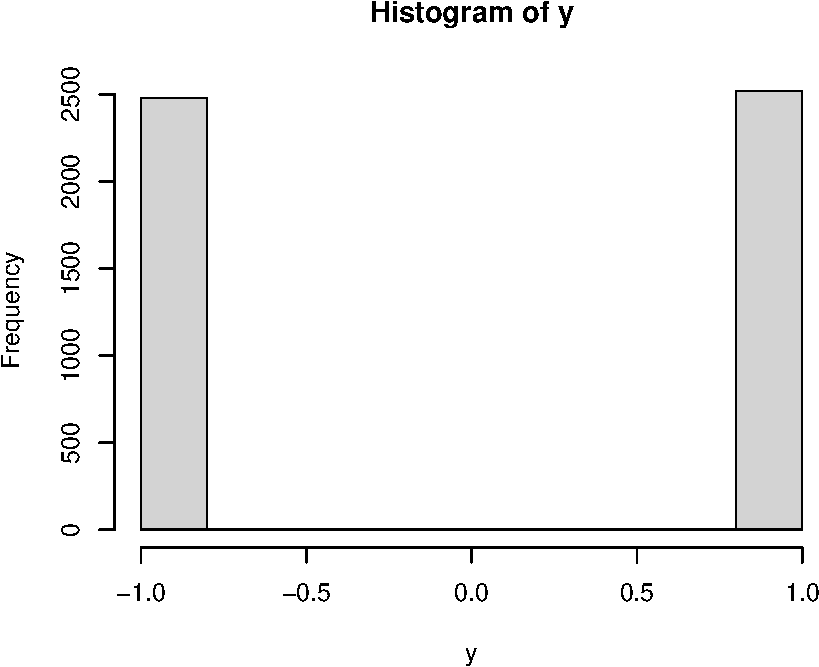
\includegraphics[width=0.5\linewidth]{RecEx4_files/figure-latex/unnamed-chunk-1-1} \end{center}

We wish to use this data set to make a prediction for \(Y\) when
\(X_1=1, X_2=2\) using the \(K\)-nearest neighbors classification
method.

\hypertarget{a}{%
\subsection{a)}\label{a}}

Calculate the Euclidean distance between each observation and the test
point, \(X_1=1,X_2=2\).

\hypertarget{b}{%
\subsection{b)}\label{b}}

Use \(P(Y=j\mid X=x_0) = \frac{1}{K}\sum_{I \in \mathcal{N}_0}I(Y=j)\)
to predict the class of \(Y\) when \(K=1\), \(K=4\) and \(K=7\). Why is
\(K=7\) a bad choice?

\hypertarget{c}{%
\subsection{c)}\label{c}}

If the Bayes decision boundary in this problem is highly non-linear,
would we expect the best value for \(K\) to be large or small? Why?

\hypertarget{problem-2-bank-notes-and-lda-with-calculations}{%
\section{Problem 2: Bank notes and LDA (with
calculations)}\label{problem-2-bank-notes-and-lda-with-calculations}}

To distinguish between genuine and fake bank notes measurements of
length and diagonal of an image part of the bank notes have been made.
For 1000 bank notes (500 genuine and 500 false) this gave the following
values for the mean and the covariance matrix (using unbiased
estimators), where the first value is the length of the bank note.

Genuine bank notes: \[
\bar{\bf x}_G=\left[     \begin{array}{c} 214.97 \\ 141.52  \end{array} \right]
\text{ and }
\hat{\boldsymbol \Sigma}_G=\left[     \begin{array}{cc} 0.1502 & 0.0055 \\ 0.0055 & 0.1998 
\end{array} \right]
\]

Fake bank notes: \[
\bar{\bf x}_F= \left[     \begin{array}{c} 214.82 \\ 139.45  \end{array} \right]
\text{ and }
\hat{\boldsymbol \Sigma}_F= \left[     \begin{array}{cc} 0.1240 & 0.0116 \\ 0.0116 & 0.3112 
\end{array} \right]
\]

\hypertarget{a-1}{%
\subsection{a)}\label{a-1}}

Assume the true covariance matrix for the genuine and fake bank notes
are the same. How would you estimate the common covariance matrix?

\hypertarget{b-1}{%
\subsection{b)}\label{b-1}}

Explain the assumptions made to use linear discriminant analysis to
classify a new observation to be a genuine or a fake bank note. Write
down the classification rule for a new observation (make any assumptions
you need to make).

\hypertarget{c-1}{%
\subsection{c)}\label{c-1}}

Use the method in b) to determine if a bank note with length \(214.0\)
and diagonal \(140.4\) is genuine or fake. You can use R to perform the
matrix calculations.

\textbf{R-hints}:

\begin{Shaded}
\begin{Highlighting}[]
\CommentTok{\# inv(A)}
\FunctionTok{solve}\NormalTok{(A)}
\CommentTok{\# transpose of vector}
\FunctionTok{t}\NormalTok{(v)}
\CommentTok{\# determinant of A}
\FunctionTok{det}\NormalTok{(A)}
\CommentTok{\# multiply vector and matrix / matrix and matrix}
\NormalTok{v }\SpecialCharTok{\%*\%}\NormalTok{ A}
\NormalTok{B }\SpecialCharTok{\%*\%}\NormalTok{ A}
\end{Highlighting}
\end{Shaded}

\hypertarget{d}{%
\subsection{d)}\label{d}}

What is the difference between LDA and QDA? Use the classification rule
for QDA to determine the bank note from c). Do you obtain the same
result? You can use R to perform the matrix calculations.

Hint: the following formulas might be useful. \[A^{-1} = \left[
\begin{array}{cc} a & b \\ c & d \end{array} 
\right]^{-1} = \frac{1}{ad-bc}
\left[
\begin{array}{cc} d & -b \\ -c & a \end{array} 
\right]\]

\[ |A| = det(A) = \Big|\begin{array}{cc} a & b \\ c & d \end{array}\Big| = ad - bc \]

\hypertarget{problem-3-odds-exercise-4.7.9-in-isl-textbook}{%
\section{Problem 3: Odds (Exercise 4.7.9 in ISL
textbook)}\label{problem-3-odds-exercise-4.7.9-in-isl-textbook}}

This problem has to do with \emph{odds}.

\hypertarget{a-2}{%
\subsection{a)}\label{a-2}}

On average, what fraction of people with an odds of \(0.37\) of
defaulting on their credit card payment will in fact default?

\hypertarget{b-2}{%
\subsection{b)}\label{b-2}}

Suppose that an individual has a \(16\%\) chance of defaulting on her
credit card payment. What are the odds that she will default?

\hypertarget{problem-4-logistic-regression-exercise-4.7.6-in-isl-textbook}{%
\section{Problem 4: Logistic regression (Exercise 4.7.6 in ISL
textbook)}\label{problem-4-logistic-regression-exercise-4.7.6-in-isl-textbook}}

Suppose we collect data for a group of students in a statistics class
with variables \(x_1\) = hours studied, \(x_2\) = undergrad grade point
average (GPA), and \(Y\) = receive an A. We fit a logistic regression
and produce estimated coefficient,
\(\hat{\beta}_0 = -6, \hat{\beta}_1 = 0.05, \hat{\beta}_2 = 1\).

\hypertarget{a-3}{%
\subsection{a)}\label{a-3}}

Estimate the probability that a student who studies for \(40\) h and has
an undergrad GPA of \(3.5\) gets an A in the class.

\hypertarget{b-3}{%
\subsection{b)}\label{b-3}}

How many hours would the student in part a) need to study to have an
estimated \(50\%\) probability of getting an A in the class?

\hypertarget{problem-5-sensitivity-specificity-roc-and-auc}{%
\section{Problem 5: Sensitivity, specificity, ROC and
AUC}\label{problem-5-sensitivity-specificity-roc-and-auc}}

We have a two-class problem, with classes 0=non-disease and 1=disease,
and a method \(p(x)\) that produces probability of disease for a
covariate \(x\). In a population we have investigated \(N\) individuals
and know the predicted probability of disease \(p(x)\) and true disease
status for these \(N\).

\hypertarget{a-4}{%
\subsection{a)}\label{a-4}}

We choose the rule \(p(x)>0.5\) to classify to disease. Define the
sensitivity and the specificity of the test.

\hypertarget{b-4}{%
\subsection{b)}\label{b-4}}

Explain how you can construct a reciever operator curve (ROC) for your
setting, and why that is a useful thing to do. In particular, why do we
want to investigate different cut-offs of the probability of disease?

\hypertarget{c-2}{%
\subsection{c)}\label{c-2}}

Assume that we have a competing method \(q(x)\) that also produces
probability of disease for a covariate \(x\). We get the information
that the AUC of the \(p(x)\)-method is 0.6 and the AUC of the
\(q(x)\)-method is 0.7. What is the definition and interpretation of the
AUC? Would you prefer the \(p(x)\) or the \(q(x)\) method for
classification?

\begin{center}\rule{0.5\linewidth}{0.5pt}\end{center}

\hypertarget{data-analysis-with-r}{%
\section{Data analysis with R}\label{data-analysis-with-r}}

For the following problems, you should check out and learn how to use
the following R functions: \texttt{glm()} (\texttt{stats} library),
\texttt{lda()}, \texttt{qda()} (\texttt{MASS} library), \texttt{knn()}
(\texttt{class} library), \texttt{roc()} and \texttt{auc()}
(\texttt{pROC} library).

\hypertarget{problem-6-exercise-4.7.10-in-isl-textbook---modified}{%
\section{Problem 6 (Exercise 4.7.10 in ISL textbook -
modified)}\label{problem-6-exercise-4.7.10-in-isl-textbook---modified}}

This question should be answered using the \texttt{Weekly} data set,
which is part of the \texttt{ISLR} package. This data is similar in
nature to the \texttt{Smarket} data from this chapter's lab, except that
it contains \(1,089\) weekly returns for \(21\) years, from the
beginning of 1990 to the end of 2010.

\hypertarget{a-5}{%
\subsection{a)}\label{a-5}}

Produce numerical and graphical summaries of the \texttt{Weekly} data.
Do there appear to be any patterns? \textbf{R-hint}: Load the data as
follows:

\begin{Shaded}
\begin{Highlighting}[]
\FunctionTok{data}\NormalTok{(}\StringTok{"Weekly"}\NormalTok{)}
\end{Highlighting}
\end{Shaded}

\hypertarget{b-5}{%
\subsection{b)}\label{b-5}}

Use the full data set to perform a logistic regression with
\texttt{Direction} as the response and the five lag variables plus
\texttt{Volume} as predictors. Use the \texttt{summary()} function to
print the results. Which of these predictors appears to be of
interest?\\
\textbf{R-hints:} You should use the \texttt{glm()} function with the
argument \texttt{family="binomial"} to make a logistic regression model.

\hypertarget{c-3}{%
\subsection{c)}\label{c-3}}

Compute the confusion matrix and overall fraction of correct
predictions. Explain what the confusion matrix is telling you about the
types of mistakes made by logistic regression.\\
\textbf{R-hints:} insert the name of your model for
\texttt{yourGlmModel} in the code below to get the predicted
probabilities for ``Up'', the classified direction and the confusion
matrix.

\begin{Shaded}
\begin{Highlighting}[]
\NormalTok{glm.probs\_Weekly }\OtherTok{\textless{}{-}} \FunctionTok{predict}\NormalTok{(yourGlmModel, }\AttributeTok{type =} \StringTok{"response"}\NormalTok{)}
\NormalTok{glm.preds\_Weekly }\OtherTok{\textless{}{-}} \FunctionTok{ifelse}\NormalTok{(glm.probs\_Weekly }\SpecialCharTok{\textgreater{}} \FloatTok{0.5}\NormalTok{, }\StringTok{"Up"}\NormalTok{, }\StringTok{"Down"}\NormalTok{)}
\FunctionTok{table}\NormalTok{(glm.preds\_Weekly, Weekly}\SpecialCharTok{$}\NormalTok{Direction)}
\end{Highlighting}
\end{Shaded}

\hypertarget{d-1}{%
\subsection{d)}\label{d-1}}

Now fit the logistic regression model using a training data period from
1990 to 2008, with \texttt{Lag2} as the only predictor. Compute the
confusion matrix and the overall fraction of correct predictions for the
held out data (that is, the data from 2009 and 2010).\\
\textbf{R-hints:} use the following code to divide into test and train
set. For predicting the direction of the test set, use
\texttt{newdata\ =\ Weekly\_test} in the \texttt{predict()} function.

\begin{Shaded}
\begin{Highlighting}[]
\NormalTok{Weekly\_trainID }\OtherTok{\textless{}{-}}\NormalTok{ (Weekly}\SpecialCharTok{$}\NormalTok{Year }\SpecialCharTok{\textless{}} \DecValTok{2009}\NormalTok{)}
\NormalTok{Weekly\_train }\OtherTok{\textless{}{-}}\NormalTok{ Weekly[Weekly\_trainID, ]}
\NormalTok{Weekly\_test }\OtherTok{\textless{}{-}}\NormalTok{ Weekly[}\SpecialCharTok{!}\NormalTok{Weekly\_trainID, ]}
\end{Highlighting}
\end{Shaded}

\hypertarget{e}{%
\subsection{e)}\label{e}}

Repeat d) using LDA.

\hypertarget{f}{%
\subsection{f)}\label{f}}

Repeat d) using QDA.

\textbf{R-hints:} plug in you variables in the following code to perform
lda and qda (just replacing \texttt{lda} with \texttt{qda}).

\begin{Shaded}
\begin{Highlighting}[]
\FunctionTok{library}\NormalTok{(MASS)}
\NormalTok{lda.Weekly }\OtherTok{\textless{}{-}} \FunctionTok{lda}\NormalTok{(Response }\SpecialCharTok{\textasciitilde{}}\NormalTok{ pred1, }\AttributeTok{data =}\NormalTok{ youTrainData)}
\NormalTok{lda.Weekly\_pred }\OtherTok{\textless{}{-}} \FunctionTok{predict}\NormalTok{(yourModel, }\AttributeTok{newdata =}\NormalTok{ YourTestData)}\SpecialCharTok{$}\NormalTok{class}
\NormalTok{lda.Weekly\_prob }\OtherTok{\textless{}{-}} \FunctionTok{predict}\NormalTok{(yourModel, }\AttributeTok{newdata =}\NormalTok{ YourTestData)}\SpecialCharTok{$}\NormalTok{posterior}
\FunctionTok{table}\NormalTok{(lda.Weekly\_pred, YourTestData}\SpecialCharTok{$}\NormalTok{Direction)}
\end{Highlighting}
\end{Shaded}

\hypertarget{g}{%
\subsection{g)}\label{g}}

Repeat d) using KNN with \(K=1\).

\textbf{R-hints:} plug in you variables in the following code to perform
KNN. The argument \texttt{prob=TRUE} will provide the probabilities for
the classified direction (which you will need later). When there are
ties (same amount of Up and Down for the nearest neighbors), the
\texttt{knn} function picks a class at random. We use the
\texttt{set.seed()} function such that we don't get different answers
for each time we run the code.

\begin{Shaded}
\begin{Highlighting}[]
\FunctionTok{library}\NormalTok{(class)}
\NormalTok{knn.train }\OtherTok{\textless{}{-}} \FunctionTok{as.matrix}\NormalTok{(YourTrainData}\SpecialCharTok{$}\NormalTok{Lag2)}
\NormalTok{knn.test }\OtherTok{\textless{}{-}} \FunctionTok{as.matrix}\NormalTok{(YourTestData}\SpecialCharTok{$}\NormalTok{Lag2)}

\FunctionTok{set.seed}\NormalTok{(}\DecValTok{123}\NormalTok{)}
\NormalTok{yourKNNmodel }\OtherTok{\textless{}{-}} \FunctionTok{knn}\NormalTok{(}\AttributeTok{train =}\NormalTok{ knn.train,}
                    \AttributeTok{test =}\NormalTok{ knn.test,}
                    \AttributeTok{cl =}\NormalTok{ YourTrainData}\SpecialCharTok{$}\NormalTok{Direction,}
                    \AttributeTok{k =}\NormalTok{ YourValueOfK,}
                    \AttributeTok{prob =} \ConstantTok{TRUE}\NormalTok{)}
\FunctionTok{table}\NormalTok{(yourKNNmodel, YourTestData}\SpecialCharTok{$}\NormalTok{Direction)}
\end{Highlighting}
\end{Shaded}

\hypertarget{h}{%
\subsection{h)}\label{h}}

Use the following code to find the best value of \(K\). Report the
confusion matrix and overall fraction of correct predictions for this
value of \(K\).

\begin{Shaded}
\begin{Highlighting}[]
\CommentTok{\#knn error:}
\NormalTok{K }\OtherTok{\textless{}{-}} \DecValTok{30}
\NormalTok{knn.error }\OtherTok{\textless{}{-}} \FunctionTok{rep}\NormalTok{(}\ConstantTok{NA}\NormalTok{, K)}

\FunctionTok{set.seed}\NormalTok{(}\DecValTok{234}\NormalTok{)}
\ControlFlowTok{for}\NormalTok{ (k }\ControlFlowTok{in} \DecValTok{1}\SpecialCharTok{:}\NormalTok{K) \{}
\NormalTok{  knn.pred }\OtherTok{\textless{}{-}} \FunctionTok{knn}\NormalTok{(}\AttributeTok{train =}\NormalTok{ knn.train,}
                  \AttributeTok{test =}\NormalTok{ knn.test,}
                  \AttributeTok{cl =}\NormalTok{ Weekly\_train}\SpecialCharTok{$}\NormalTok{Direction,}
                  \AttributeTok{k =}\NormalTok{ k)}
\NormalTok{  knn.error[k] }\OtherTok{\textless{}{-}} \FunctionTok{mean}\NormalTok{(knn.pred }\SpecialCharTok{!=}\NormalTok{ Weekly\_test}\SpecialCharTok{$}\NormalTok{Direction)}
\NormalTok{\}}
\NormalTok{knn.error.df }\OtherTok{\textless{}{-}} \FunctionTok{data.frame}\NormalTok{(}\AttributeTok{k =} \DecValTok{1}\SpecialCharTok{:}\NormalTok{K, }\AttributeTok{error =}\NormalTok{ knn.error)}
\FunctionTok{ggplot}\NormalTok{(knn.error.df, }\FunctionTok{aes}\NormalTok{(}\AttributeTok{x =}\NormalTok{ k, }\AttributeTok{y =}\NormalTok{ error)) }\SpecialCharTok{+}
  \FunctionTok{geom\_point}\NormalTok{(}\AttributeTok{col =} \StringTok{"blue"}\NormalTok{) }\SpecialCharTok{+}
  \FunctionTok{geom\_line}\NormalTok{(}\AttributeTok{linetype =} \StringTok{"dotted"}\NormalTok{)}
\end{Highlighting}
\end{Shaded}

\hypertarget{i}{%
\subsection{i)}\label{i}}

Which of these methods appear to provide the best results on this data?

\hypertarget{j}{%
\subsection{j)}\label{j}}

Plot the ROC curves and calculate the AUC for the four methods (using
your the best choice for KNN). What can you say about the fit of these
models?

\textbf{R-hints}:

\begin{itemize}
\tightlist
\item
  For KNN you can use \texttt{knn(...,prob=TRUE)} to get the probability
  for the classified direction. Note that we want \(P(Direction = Up)\)
  when plotting the ROC-curve, so we need to modify the probabilties
  returned from the \texttt{knn} function.
\end{itemize}

\begin{Shaded}
\begin{Highlighting}[]
\CommentTok{\#get the probabilities for the classified class}
\NormalTok{yourKNNProbs }\OtherTok{\textless{}{-}} \FunctionTok{attributes}\NormalTok{(yourKNNmodel)}\SpecialCharTok{$}\NormalTok{prob}

\CommentTok{\# since we want the probability for Up, we need to take 1{-}p for the elements}
\CommentTok{\# that gives probability for Down}
\NormalTok{down }\OtherTok{\textless{}{-}} \FunctionTok{which}\NormalTok{(yourKNNmodel }\SpecialCharTok{==} \StringTok{"Down"}\NormalTok{)}
\NormalTok{yourKNNProbs[down] }\OtherTok{\textless{}{-}} \DecValTok{1} \SpecialCharTok{{-}}\NormalTok{ yourKNNProbs[down]}
\end{Highlighting}
\end{Shaded}

\begin{itemize}
\tightlist
\item
  Use the following code to produce ROC-curves:
\end{itemize}

\begin{Shaded}
\begin{Highlighting}[]
\CommentTok{\#install.packages("plotROC")}
\CommentTok{\#install.packages("pROC")}
\FunctionTok{library}\NormalTok{(pROC)}
\FunctionTok{library}\NormalTok{(plotROC)}

\NormalTok{yourRoc }\OtherTok{\textless{}{-}} \FunctionTok{roc}\NormalTok{(}\AttributeTok{response =}\NormalTok{ Weekly\_test}\SpecialCharTok{$}\NormalTok{Direction,}
               \AttributeTok{predictor =}\NormalTok{ yourModelsPredictedProb,}
               \AttributeTok{direction =} \StringTok{"\textless{}"}\NormalTok{)}
\CommentTok{\#you can use this function for all your methods and plot them using plot(yourRoc)}

\CommentTok{\#or use ggplot2 }
\NormalTok{dat }\OtherTok{\textless{}{-}} \FunctionTok{data.frame}\NormalTok{(}\AttributeTok{Direction =}\NormalTok{ Weekly\_test}\SpecialCharTok{$}\NormalTok{Direction,}
                 \AttributeTok{glm =}\NormalTok{ yourGlmProbs, }
                 \AttributeTok{lda =}\NormalTok{ yourLDAProbs[, }\DecValTok{2}\NormalTok{],}
                 \AttributeTok{qda =}\NormalTok{ yourQDAProbs[, }\DecValTok{2}\NormalTok{],}
                 \AttributeTok{knn =}\NormalTok{ yourKNNProbs)}
\NormalTok{dat\_long }\OtherTok{\textless{}{-}} \FunctionTok{melt\_roc}\NormalTok{(dat, }\StringTok{"Direction"}\NormalTok{, }\FunctionTok{c}\NormalTok{(}\StringTok{"glm"}\NormalTok{, }\StringTok{"lda"}\NormalTok{, }\StringTok{"qda"}\NormalTok{, }\StringTok{"knn"}\NormalTok{))}
\FunctionTok{ggplot}\NormalTok{(dat\_long, }\FunctionTok{aes}\NormalTok{(}\AttributeTok{d =}\NormalTok{ D, }\AttributeTok{m =}\NormalTok{ M, }\AttributeTok{color =}\NormalTok{ name)) }\SpecialCharTok{+}
  \FunctionTok{geom\_roc}\NormalTok{(}\AttributeTok{n.cuts =} \ConstantTok{FALSE}\NormalTok{) }\SpecialCharTok{+}
  \FunctionTok{xlab}\NormalTok{(}\StringTok{"1{-}Specificity"}\NormalTok{) }\SpecialCharTok{+}
  \FunctionTok{ylab}\NormalTok{(}\StringTok{"Sensitivity"}\NormalTok{)}
\CommentTok{\#glm is very similar to lda, so the roc{-}curve for glm is not shown. }

\CommentTok{\#AUC: yourAUC = auc(yourRoc)}
\end{Highlighting}
\end{Shaded}


\end{document}
